\chapter{Markov Kette} 
\label{mainsec:mk}
Grundlage des Hidden Markov Model war die vom russischen Mathematiker Andrej Andrejewitsch Markov 
(1856 - 1922, siehe \cite{markov1913}) entwickelte Markov Kette. Zu Beginn des 20. Jahrhunderts beschäftigte er sich als erster mit einer statistischen Beschreibung von Zustands- und Symbolfolgen. Er führte eine statistische Analyse der Buchstabenfolge des Textes ``Eugene Onegin'' von Alexander Pushkin durch.


\section{Beispiel} 
\textit{ Markov Kette für das Wetter \footnote{Quelle: \url{en.wikipedia.org/wiki/Examples_of_Markov_chains}}} \\
Im folgenden Beispiel soll aufgrund des aktuellen Wetters auf das Wetter der folgenden Tage geschlossen werden.
Das Wetter kann entweder ``sunny'' oder ``rainy'' sein, zu Beginn (Tag 0, \( t = 0 \)) des Experiments ist es ``sunny''.
Die Wahrscheinlichkeit, dass auf ``sunny'' wieder ``sunny'' folgt, liegt bei 90\% (``rainy'' = 1 - ``sunny'' = 10\%). 
Nach ``rainy'' liegt die Wahrscheinlichkeit jeweils bei 50\% (siehe Abb. \ref{fig:simple_mc_example}).  
\begin{figure}[htbp] \centering
    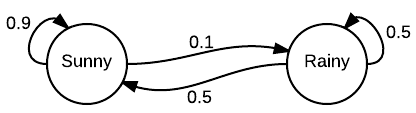
\includegraphics[width=0.5\textwidth]{Bilder/Kap2/simple_mc_example.png}
    \caption{ Gerichteter Zustandsgraph der modellierten Wetter-Markov Kette }
    \label{fig:simple_mc_example}
\end{figure}


\[ Zust\ddot{a}nde: S = [``sunny'', ``rainy''] \]
\[ Anfangszustand:  \Pi = X_0 = [1 , 0] \]
\[\ddot{U}bergangsmatrix: A = \begin {bmatrix} 0.9&0.1\\0.5&0.5 \end {bmatrix}
\]

Nun kann die Wahrscheinlichkeit für das Wetter an Tag 1 berechnet werden über: \\
\[ X_1 = X_0 * A = [ 1, 0 ] \begin {bmatrix} 0.9&0.1\\0.5&0.5 \end {bmatrix} = [ 0.9, 0.1] \]

Für Tag 2:\\
\[ X_2 = X_1 A = X_0 A^2 = [ 1, 0 ] \begin {bmatrix} 0.9&0.1\\0.5&0.5 \end {bmatrix}^2 = [ 0.86, 0.14] \] 

Verallgemeinert für Tag k bedeutet das: 
\[ X_k = X_{k-1} A = X_0 A^k = [ 1, 0 ] \begin {bmatrix} 0.9&0.1\\0.5&0.5 \end {bmatrix}^k \] 


\section{Definition}
Eine Markov Kette beschreibt einen zeit-diskreten Prozess \((X_t)_{t\in\mathbb{N}_0}\) mit  \(m\) abzählbaren Zuständen \(S\) \cite{stochMod}.
Weiterhin wird sie als stationär bezeichnet, wenn alle Wahrscheinlichkeiten unabhängig von der Zeit sind.
Da die Verteilung der Zufallsvariablen nur von den vergangenen Zuständen abhängt, gilt eine Markov Kette als kausal \cite[48]{mmmFink}.
Definition \ref{equ:markov} zeigt die allgemeine Berechnung der Übergangswahrscheinlichkeiten einer Markov Kette. Als Übergangswahrscheinlichkeit bezeichnte man die bedingte Wahrscheinlichkeit \(P ( X_{t+1} = s_{t+1} | X_{t} = s_{t} ) \), sodass auf 
den aktuellen Zustand \( s_{t}\) der Nachfolgezustand \( s_{t+1}\) folgt. 
\begin{equation}
\label{equ:markov}
P (X_{t+1} = s_{t+1} | X_0 = s_0, \ldots , X_{t-1} = s_{t-1}, X_{t} = s_{t})
\end{equation}

Wichtig für eine Markov Kette ist die sog. Markov-Eigenschaft (Siehe Gleichung \ref{equ:markovProp}). Im Unterschied zu Gleichung \ref{equ:markov} hängt der nächste Zustand nur vom aktuellen Zustand ab. 
\begin{equation}
\label{equ:markovProp}
P ( X_{t+1} = s_{t+1} | X_{t} = s_{t} ) 
\end{equation}
Genügt eine Markov Kette dieser Eigenschaft, wird sie als ``einfach'' oder Markov Kette 1. Ordnung bezeichnet.
Anders ausgedrückt beschreibt die Markov-Eigenschaft die Gedächtnislosigkeit des Prozesses, da der Folgezustand nur vom direkten Vorgänger abhängt.

Die Übergangswahrscheinlichkeiten werden üblicherweise zu einer Übergangsmatrix zusammengefasst (Definition \ref{equ:markovTrans}) 

\begin{equation}
\label{equ:markovTrans}
A = [a_{ij}] =
\begin {bmatrix} 
  a_{00}&\cdots&a_{0m} \\
  \vdots&\ddots&\vdots \\
  a_{m0}&\cdots&a_{mm}
 \end {bmatrix} \forall i, j \in S
\end{equation}
Da es sich um Wahrscheinlichkeiten handelt, muss sich die Summe jeder Reihe zu Eins addieren. \\

Weiterhin benötigt der Prozess einen Vektor für den Anfangzustand $t = 0$ (Definiton \ref{equ:markovStart})
\begin{equation}
 \label{equ:markovStart}
 \Pi = [ \pi_i] = [ P (X_0 = i) ] , i \in S
\end{equation}

So lässt sich eine Markov-Kette durch Zustandsraum \(S\), den Übergangsmatrix \( A \) und einen Anfangszustand \( \Pi \) definieren.

Veranschaulichen lässt sich eine Markov Kette als gerichtetes Zustandsdiagramm (Abb. \ref{fig:simple_mc}) mit den Zuständen \(S\) und 
mit den Übergangswahrscheinlichkeiten \(X_i\) an den Kanten
\begin{figure}[htbp] \centering
    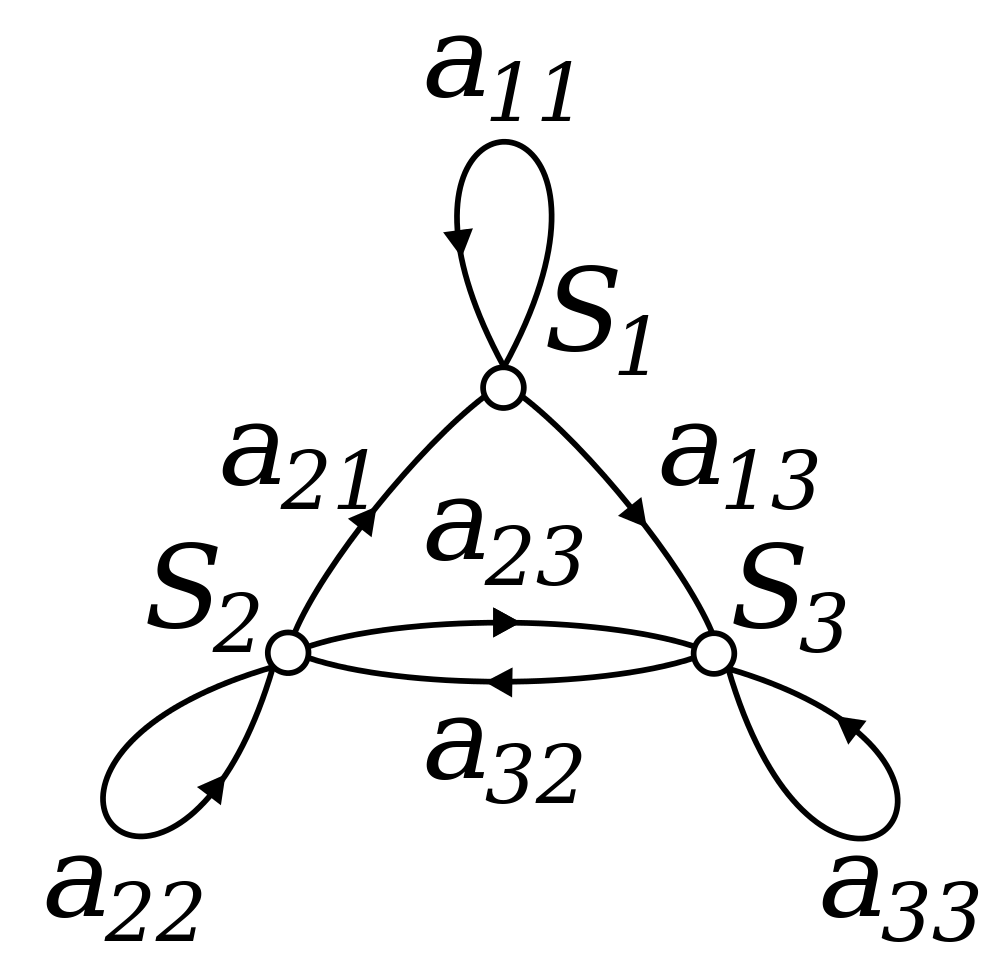
\includegraphics[width=0.5\textwidth]{Bilder/Kap2/simple_mc.png}
    \caption{Einfaches Zustandsdiagramm einer Markov Kette (Quelle: \url{de.wikipedia.org/wiki/Markow-Kette})}
    \label{fig:simple_mc}
\end{figure}

Die Wahrscheinlichkeit für \( k \)-Schritte lässt sich so ausrechnen: 
\[ X_k = X_{k-1} A = X_0 A^k \] 
